\chapter{ВЫПОЛНЕНИЕ ЗАДАНИЯ}
Необходимо разработать программу для ПЛК для управления автоматизированной
установкой в соответствии с описанием ее работы.

\textbf{Цель} --- Сделать программу для управления автоматизированной установкой в соответствии с описанием ее работы.

При выполнении ставятся следующие задачи:
\begin{enumerate}
    \item Внимательно ознакомиться с заданием
    \item Изучить алгоритм работы установки
    \item Изучить электрическую схему подключения
    \item Изучить пневматическую схему подключения
    \item Определить сигналы для выполнения исполнительных элементов
    \item Создать программу для управления установкой
\end{enumerate}

Автоматическая установка состоит из трех пневматических цилиндров, шести
датчиков положения (герконы), одного двигателя постоянного тока и световой
колонны. Всеми перемещениями механизмов и индикацией световой колонны
управляет ПЛК (программируемый логический контроллер/программируемое
реле). Используется ПЛК ОВЕН ПР200-24 1.X.
Для реализации панели оператора используется встроенный scada система.

\section{Виртуальная панель оператора}
Виртуальная панель оператора в scada системе представлена на рисунке \ref{fig:scada_panel}.
\begin{figure}[hb]
    \centering
    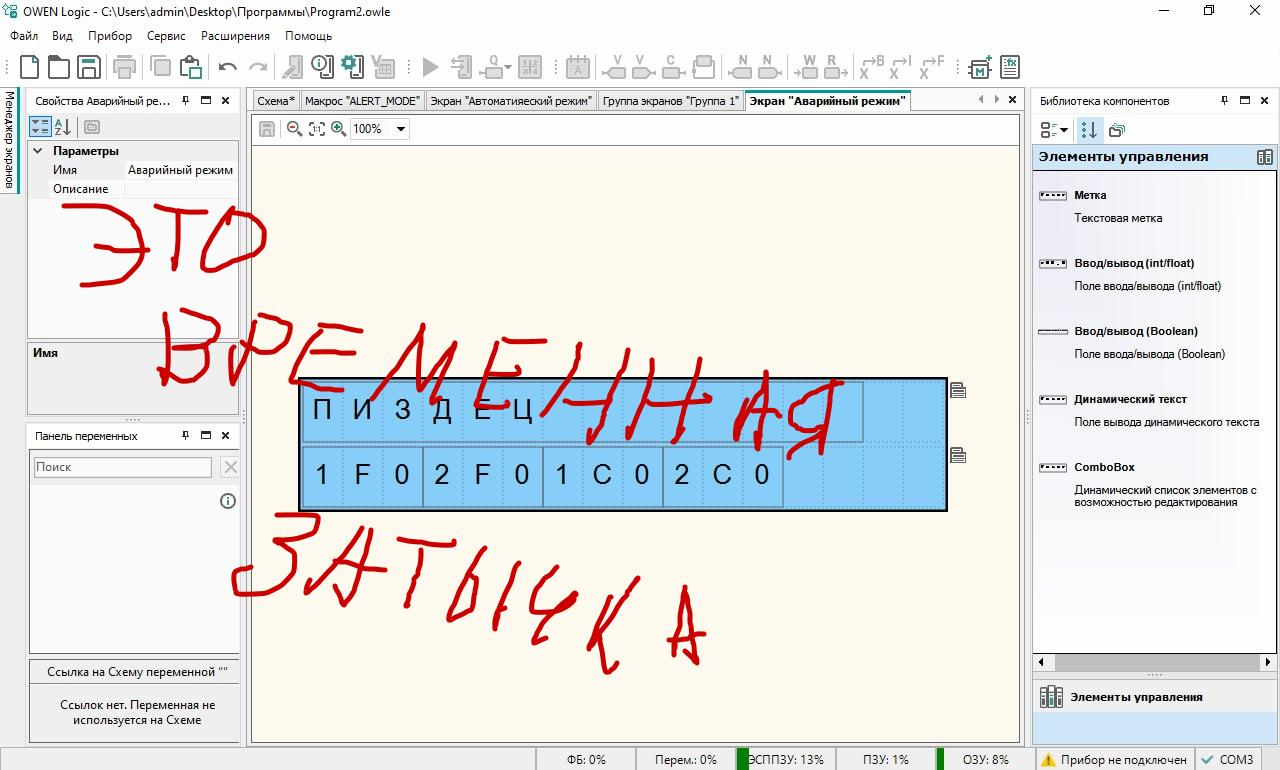
\includegraphics[scale=0.30]{fig/4.1.jpg}
    \caption{Виртуальная панель оператора}
    \label{fig:scada_panel}
\end{figure}

\subsection{Описание клавиш панели оператора}
\begin{enumerate}
    \item F1 -- аварийный останов (1 – активация)
    \item F2 -- ручной/авто (0 – ручной, 1 – автоматический)
    \item F3 -- старт (авто) / движение выбранного цилиндра (ручной)
    \item F4 -- движение выбранного цилиндра (ручной)
    \item С1 -- выбор цилиндра 1 (ручной)
    \item С2 -- выбор цилиндра 2 (ручной)
    \item С3 -- выбор цилиндра 3 (ручной)
    \item С4 -- включение двигателя (ручной)
\end{enumerate}

Из кнопок F1, F2, С1, С2, С3, С4 необходимо сделать переключатели
программным способом.

\section{Условия запуска установки}
\begin{itemize}
    \item Штекер вставлен в розетку и ручной пневматический клапан открыт для подачи воздуха в систему.
    \item Все компоненты должны оставаться в своих стартовых позициях, цилиндры 1, 2 и 3 втянуты, двигатель выключен.
    \item Выбор режима работы автоматический/ручной может быть осуществлен переключателем F2.
    \item Установка начинает свою работу только если кнопка аварийного останова F1 не активирована.
\end{itemize}



